%!TEX TS-program = xelatex
%!TEX encoding = UTF-8 Unicode

\documentclass[a4paper,11pt,fleqn]{article}
\usepackage{graphicx,url}
\usepackage[T1]{fontenc}
\usepackage[brazil]{babel}
\usepackage{a4wide}
\usepackage{booktabs}
\usepackage[table,xcdraw]{xcolor}
\usepackage{amsmath} % For math
\usepackage{fontspec}
\graphicspath{{./images/}}
\setmainfont{Times New Roman}

\title{\vspace{-4cm}Avaliação de Desempenho do Crivo Paralelo \\ {\small Computação Paralela}}
\author{Luiz Junio Veloso Dos Santos $-$ Matricula: 624037}

\begin{document}
\maketitle

% Please add the following required packages to your document preamble:
% \usepackage{graphicx}
% \usepackage[table,xcdraw]{xcolor}
% If you use beamer only pass "xcolor=table" option, i.e. \documentclass[xcolor=table]{beamer}
\begin{table}[h!]
\caption{Comparativo das métricas de performance do programa Perf.}
\centering
\resizebox{.8\textwidth}{!}{%
\begin{tabular}{|llll|}
\hline
\rowcolor[HTML]{91D39B} 
\textbf{Contador} & \textbf{Sequencial} & \textbf{\begin{tabular}[c]{@{}l@{}}Paralelo\\ (Dinâmico)\end{tabular}} & \textbf{\begin{tabular}[c]{@{}l@{}}Paralelo\\ (Estático)\end{tabular}} \\ \hline
\multicolumn{1}{|l|}{\textbf{CPUs utilized}} & 1 & 1,97 & 1,97 \\
\rowcolor[HTML]{CCCCCC} 
\multicolumn{1}{|l|}{\cellcolor[HTML]{CCCCCC}\textbf{frontend cycles idle}} & n/a & n/a & n/a \\
\multicolumn{1}{|l|}{\textbf{backend cycles idle}} & n/a & n/a & n/a \\
\rowcolor[HTML]{CCCCCC} 
\multicolumn{1}{|l|}{\cellcolor[HTML]{CCCCCC}\textbf{instructions per cycle}} & 0,65 & 0,33 & {\color[HTML]{333333} 0,33} \\
\multicolumn{1}{|l|}{\textbf{LL-cache hits}} & 12,36\% & 3,87\% & 6,42\% \\
\rowcolor[HTML]{CCCCCC} 
\multicolumn{1}{|l|}{\cellcolor[HTML]{CCCCCC}\textbf{time elapsed}} & 1,43 seg & 1,218 seg & 1,206 seg \\ \hline
\end{tabular}%
}
\label{tab:my-table}
\end{table}

O maior gargalo desse programa está sendo no seu \textit{for} externo,
que não foi paralelizado na tarefa 07, o que resultou na diminuição
do número de instruções por ciclo, por fazer menos processamento.

Havia paralelizado apenas o \textit{for} interno por acreditar, que dado o
funcionamento do Crivo de Aristóteles, eu não poderia ``remover''
os múltiplos, por exemplo 2,4,8 e uma outra thread acessar uma posição
como a 4, que foi ``removida''. 

Mas como essa implementação usa de valores booleanos e não remoção uma
remoção física do valor em uma posição do array, não irá ocorrer problema.
Contudo se então eu paralelizar o \textit{for} externo, na teoria, terei um aumento nas instruções por ciclo, mas também um aumento do tempo, uma vez que estarei
possivelmente acessando mais vezes o \textit{for} interno.

Uma melhoria seria aumentar o número de threads para 4, e experimentar
diferentes politicas de escalonamento.

\newpage
\begin{figure}[h!]
    \caption{Código utilizado com as primitivas OpenMP}
    \centering
    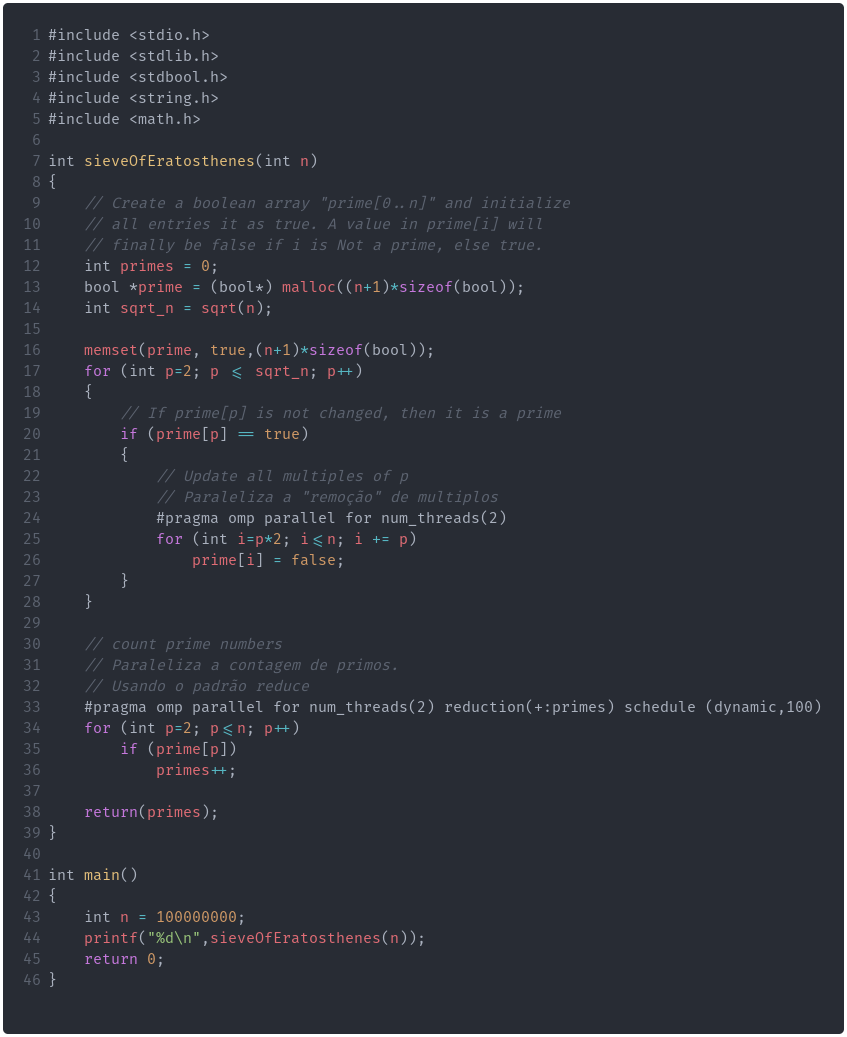
\includegraphics[scale=0.56]{carbon}
\end{figure}

\end{document}
